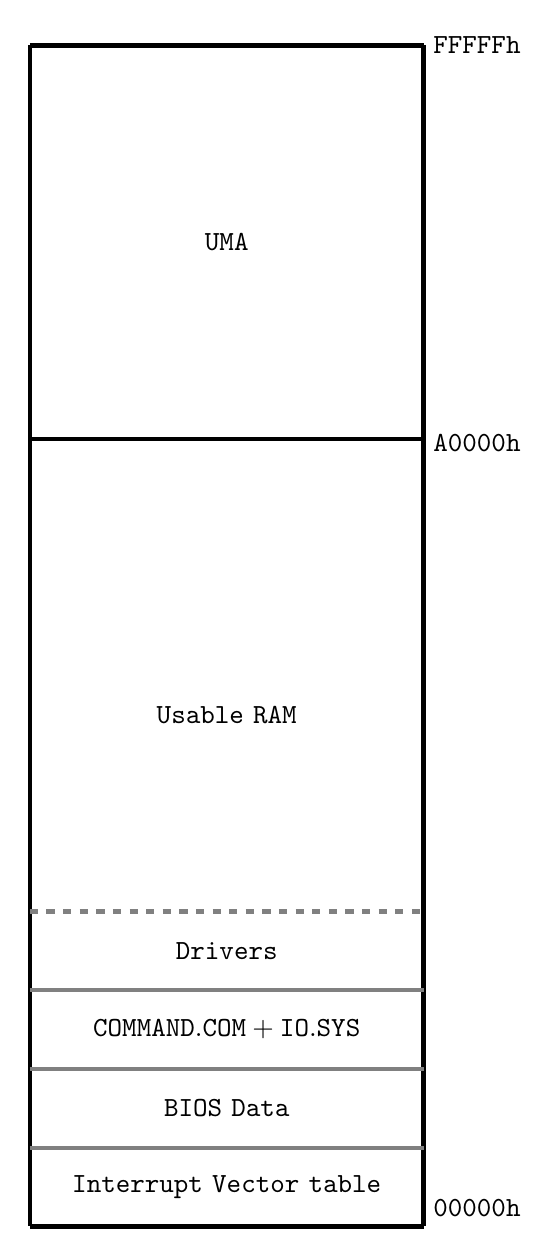
\begin{tikzpicture}


%Draw borders of ALL RAM
\draw[ultra thick,black] (5,0)  -- (0,0);
\draw[ultra thick,black] (5,0 ) -- (5,15);
\draw[ultra thick,black] (0,15) -- (5,15);
\draw[ultra thick,black] (0,15)  -- (0,0);

%Defining grey color
\colorlet{LighterMark}{black!50}

%Interrupt Vector table
\draw[ultra thick,LighterMark] (0,1)  -- (5,1);
\node[] at (2.5,0.5){$\mathtt{Interrupt\ Vector\ table}$}  ;


\node[above right,align=left] at (5,0){$\mathtt{00000h}$}  ;

%BIOS data
\draw[ultra thick,LighterMark] (0,2)  -- (5,2);
\node[] at (2.5,1.5){$\mathtt{BIOS\ Data}$}  ;

%COMAMND.COM + IO.SYS
\draw[ultra thick,LighterMark] (0,3)  -- (5,3);
\node[] at (2.5,2.5){$\mathtt{COMMAND.COM + IO.SYS}$}  ;

%Drivers
\draw[ultra thick,dashed,LighterMark] (0,4)  -- (5,4);
\node[] at (2.5,3.5){$\mathtt{Drivers}$}  ;

%Usable RAM
\node[] at (2.5,6.5){$\mathtt{Usable\ RAM}$}  ;

%UMA
\draw[ultra thick,black] (0,10)  -- (5,10);
\node[right,align=left] at (5,9.95){$\mathtt{A0000h}$}  ;
\node[] at (2.5,12.5){$\mathtt{UMA}$}  ;

%Top RAM
\node[right,align=left] at (5,15){$\mathtt{FFFFFh}$}  ;

%Braces
%\draw [decorate,decoration={brace,amplitude=10pt,mirror,raise=4pt},yshift=0pt]
%(5,0) -- (5,10) node [black,midway,xshift=0.8cm] {\footnotesize
%$XXXX$};

\end{tikzpicture}